\documentclass{article}
\usepackage[utf8]{inputenc}
\usepackage{xcolor}\usepackage{natbib}
\usepackage{graphicx}
\usepackage{float}
\usepackage{subfig}
\usepackage{blindtext}
\usepackage{hyperref}
\graphicspath{{./images/}}
\hypersetup{
    colorlinks=true,
    linkcolor=blue,
    filecolor=blue,      
    urlcolor=blue  
    }
    
\urlstyle{same}

\title{\textbf{Purple Architecture}}
\author{Joris Putteneers}
\date{June 2022}



\begin{document}


\maketitle

\section{Introduction}
it will instantly disappear and be replaced by something even more bizarre and inexplicable \cite{databaseII}.


\section{Abstract}
Lorem Ipsum ised in the 1960s with the release of Letraset sheets containing Lorem Ipsum passages, and more recently with desktop publishing software like Aldus PageMaker including {\color{blue}\LaTeX\ text} \\ 

\begin{figure}[H]
  \centering
  % \captionsetup{}
  \captionsetup{font=small,justification=raggedright,singlelinecheck=false}
  \includegraphics[width=12.8cm]{g.png}
  \caption{pointcloud model. \href{https://sketchfab.com/3d-models/wifi-workspace-visualisation-aefe16a1f9bd4296941e099754eaacc2}{sketchfab Model}.}
  \label{fig:method}
\end{figure}



\begin{figure}[H]
  % \centering
  \captionsetup{font=small,justification=raggedright,singlelinecheck=false}
  \parbox{6cm}{
  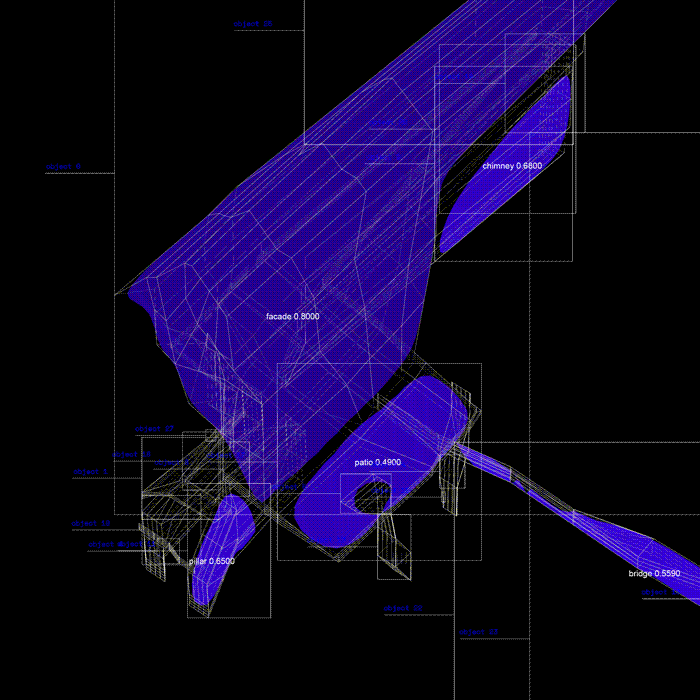
\includegraphics[width=6cm]{b.png}
  % \captionsetup{font={small,sc,onehalfspacing,color=red}}
  \caption{Object detection.}
  \label{fig:2figsA}}
  \qquad
  \begin{minipage}{6cm}
  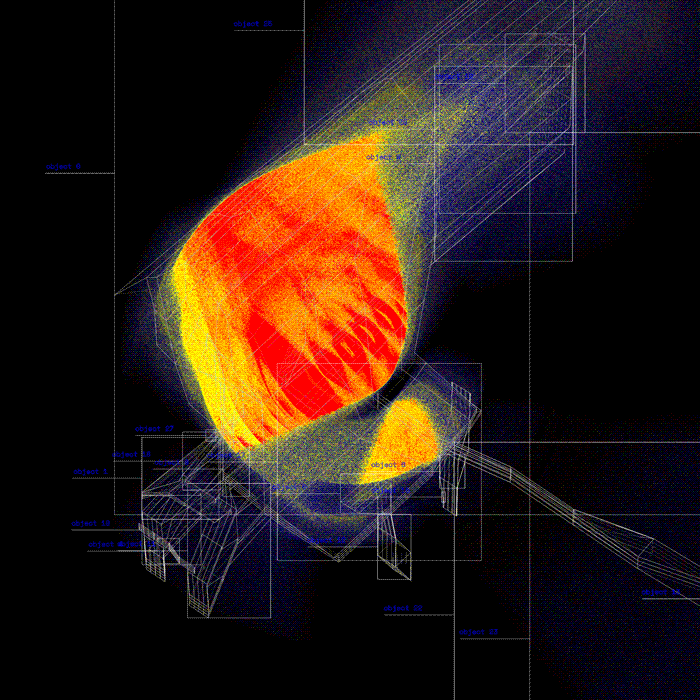
\includegraphics[width=6cm]{a.png}
  \caption{Machine vision iteration.}
  \label{fig:2figsB}
  \end{minipage}
\end{figure}






\section{Conclusion}
``I always thought something was fundamentally wrong with the universe'' \citep{adams1995hitchhiker}\\
DSFdsfdsFfdsfdsfdffsfdsfdf

\bibliographystyle{plain}
% \bibliography{references}
\end{document}